\chapter{Umsetzung der Softwarelösung}
\label{chap:umsetzung_des_prototyps}

Basierend auf den vorgestellten Konzepten folgt die technische Erläuterung der Anwendung.

\section{Implementierung des Machine Learning Modells}

\subsection{Fine-tuning der Transfomer Modelle}

Für das \textit{fine-tuning} (Training) der verschiedenen Modelle werden die Transformers-Bibliothek von Hugging Face, Python und das Deep-Learning-Framework PyTorch verwendet.

Trainiert werden fünf verschiedene Transformer Modelle mit dem Datensatz aus Kapitel \ref{sec6:datenvorverarbeitung}:
\begin{itemize}
    \item Bert base
    \item RoBERTa base
    \item RoBERTa large
    \item XML-RoBERTa base
    \item XML-RoBERTa large
\end{itemize}

In \ref{tab:bert_models} angehängt, findet sich ein tabellarischer Vergleich der verschiedenen BERT- und RoBERTa-Modelle mit deren jeweiligen technischen Eigenschaften.

Das Tokenisieren erfolgt über den jeweiligen mitgelieferten Tokenizer.

Eine Übersicht der für das \textit{fine-tuning} genutzten Hyperparameter findet sich im Anhang (siehe Tabelle \ref{tab:transformer-hyperparameter}).

Zur dynamischen Anpassung der Lernrate während des Trainings, wird ein linearer Learning Rate Scheduler mit Warmup verwendet.
Zu Beginn des Trainings wird die Lernrate über 10\% der Trainingsschritte schrittweise erhöht, um das Modell zu stabilisieren. 
Anschließend wird sie linear bis zum Ende des Trainings wieder abgesenkt. Dieses Vorgehen hilft dabei, Konvergenzprobleme zu vermeiden und die Modellleistung zu verbessern.
Konvergenzprobleme entstehen, wenn das Modell beim Training nicht richtig lernt und die Fehler (\textit{loss}) nicht zuverlässig kleiner werden.

Das Training wird auf einer Google Colab Laufzeit mit einer A100 GPU mit erweitertem RAM Speicher durchgeführt.
Die trainierten Modelle werden jeweils als einzelnen Repository im Hugging Face Hub gespeichert.

\subsection{Erzeugung der Embeddings} \label{sec:erzeugung_der_embeddings}

Für das Erzeugen der Embeddings wird der Datensatz aus Kapitel \ref{sec6:datenvorverarbeitung} in Trainings- (80\%) und Testdaten (20\%) aufgeteilt und tokenisiert.

Diese Datensätze durchlaufen anschließend folgende Schritte: 

\begin{enumerate}
  \item \textbf{Vorbereitung des Modells:}  
  Das Transformer Modell wird in den Evaluationsmodus gesetzt und auf die A100 GPU verschoben, um eine effiziente Berechnung sicherzustellen.

  \item \textbf{Erstellung eines \textit{DataLoaders}:}  
    Die tokenisierten Eingabesequenzen (bestehend aus \texttt{input\_ids}, \texttt{attention\_mask} und \texttt{labels}) werden zu Batches zusammengefügt,
    welche von der GPU parallel verarbeitet werden können. Diese werden in einem sogenannten, von \textit{PyTorch} zur Verfügung gestelltem, \textit{DataLoader} gespeichert.

  \item \textbf{Vorwärtspass:}  
  Die Batches des \textit{DataLoaders} werden in das Modell eingespeist, um Vorhersagen bzw. Zwischenrepräsentationen zu berechnen.
  Hierbei wird keine Gradientenberechnung (Backpropagation) durchgeführt, das Modell lernt also nicht von den Eingaben.

  \item \textbf{Extraktion der \textit{hidden states}:}  
  Für jedes Batch wird die Ausgabe aller versteckten Schichten (\texttt{hidden layer}) der Tranformer Modelle berechnet. 
  Jedes \textit{hidden layer} erzeugt einen \textit{hidden state}

  \item \textbf{Pooling über die letzten vier Schichten:}  
  Die letzten vier \textit{hidden state}-Schichten werden ausgewählt und über eine Mittelwertbildung (Average Pooling) zusammengefasst, 
  um eine robustere Token-Repräsentation zu erhalten.

  \item \textbf{Maskierung und Mittelung über Tokens:}  
  Mithilfe der \texttt{attention\_mask} werden \texttt{[PAD]}-Tokens ausgeschlossen. 
  Die verbleibenden Token-Embeddings werden über die Sequenzlänge gemittelt, sodass ein einziger Vektor pro Eingabesequenz entsteht.

  \item \textbf{Speicherung der Embeddings:}  
  Die resultierenden Satz-Embeddings sowie die zugehörigen Labels werden gesammelt und in \textit{NuMpy}-Arrays konvertiert.

  \item \textbf{Finaler Output:}  
  Nach Verarbeitung aller Batches werden die Satz-Embeddings und Labels aller Beispiele zu zwei großen Arrays (Embeddings und Label) zusammengefügt.
\end{enumerate}

Nach Durchlaufen der Schritte werden die Embeddings und Label der Trainings- und Testdaten in einem Python Dictionary gespeichert.

\subsection{Nutzung der Embeddings im LightGBM Modell}

Die Python LightGBM-Bibliothek stellt ein einfach zu implementierendes Modell zur Verfügung.
Dieses wird auf den verschiedenen erzeugten Embeddings trainiert.

Eine Übersicht der im Modell genutzten Hyperparameter findet sich im Anhang (siehe Tabelle \ref{tab:lightgbm-hyperparameter}).
Zur Wahl der geeignetsten Hyperparameter wird einmalig die Optuna-Bibliothek genutzt.
Dabei werden mithilfe von K-Fold-Cross-Validation (siehe Abbildung \ref{fig:k-fold_cross-validation}) verschiedene Kombinationen von LightGBM-Hyperparametern getestet, 
um das Modell mit dem höchsten F1-Score zu finden.

\begin{figure}[htbp]
    \begin{center}
        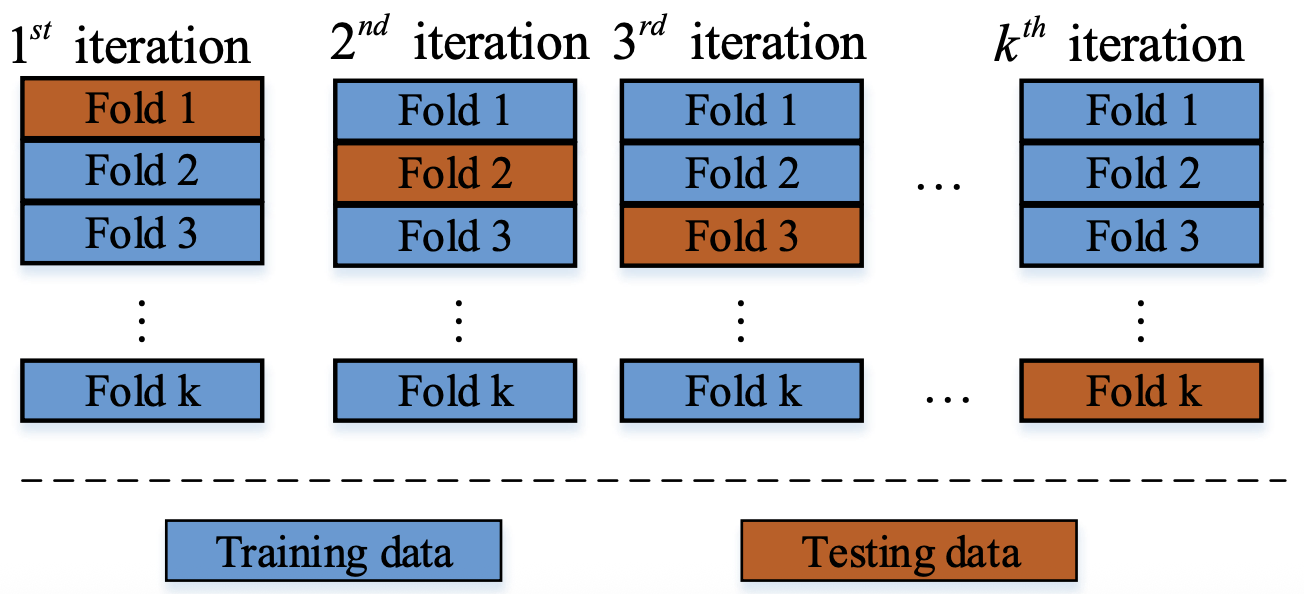
\includegraphics[scale=0.4]{static/k-fold_cross-validation.png}
        \caption{\label{fig:k-fold_cross-validation} K-Fold-Cross-Validation \cite{isaac2021}}
    \end{center}
\end{figure}

Anhand von dem, in der Bibliothek zur Verfügung gestellten, \textit{early-stopping} wird das Training des Modells überwacht und frühzeitig gestoppt, wenn bestimmte 
Anforderungen erreicht sind. 
Die Parameter sind in diesem Fall so definiert, dass das Training beendet wird, sobald sich der logarithmische Verlust (\textit{Logloss}) auf den 
Validierungsdaten über 100 aufeinanderfolgende Iterationen hinweg nicht mehr verbessert.
Dadurch wird Overfitting verhindert und eine bessere Generalisierung auf unbekannte Texte ermöglicht.

\subsection{Gesamtarchitektur}

Der Webserver wird mit der Python Starlette-Bibliothek implementiert und mit Docker containerisiert.
Nach dem Starten werden zuerst die Transformer und LightGBM Modelle geladen, danach wird das \textit{ready}-Flag gesetzt und der Server kann Anfragen empfangen.
Die einzige Klasse ist das Singleton \textit{EmbeddingService} (siehe Abbildung \ref{fig:uml_webserver}). Dieses erzeugt das Embedding und klassifiziert es anschließend.
Zurückgegeben wird ein \textit{json}-Objekt mit den Informationen \textit{label} und \textit{probability}. Das \textit{label} enthält den klassifizierten Binärwert 
(1 bedeutet Fake, 0 bedeutet Echt). Die \textit{probability} enthält die Wahrscheinlichkeit der korrekten Klassifizierung in Prozent.

\begin{figure}[htbp]
    \begin{center}
        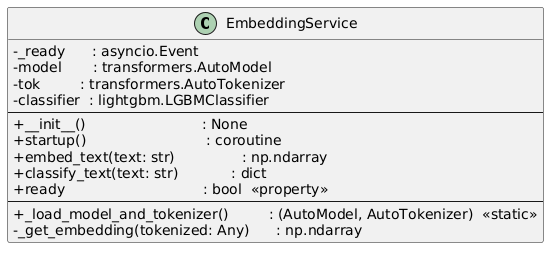
\includegraphics[scale=0.55]{static/uml_webserver.png}
        \caption{\label{fig:uml_webserver} UML des Webservers}
    \end{center}
\end{figure}

Eine Modellierung der Architektur des Webservers findet sich im Anhang \ref{fig:gesamtarchitektur}.

\section{Implementierung des Webagenten}

Zur Bestimmung des geeignetsten Tools für den Webagenten,
wurden verschiedene Technologien verglichen (siehe Tabelle \ref{table:technischeAnsaetze}).
Aufgrund des begrenzten Zugriffs auf die zu analysierende Seiten, bieten sich die beiden Client-seitigen Umsetzungen 
eine Chrome Extension zu implementieren oder über Tampermonkey Userscripts auszuführen am ehesten an.

Im Vergleich zu Usercripts unterstützt die Extension mehrere Komponenten (Content Scripts, Background Scripts, Popup, Optionsseite).
Anhand dieser können der DOM beobachtet, ein persistenter Speicher genutzt, Kontextmenüs erstellt und auf Browseraktionen reagiert werden (z.B. Tabwechsel, Navigation).
Ein Userscript hingegen ist ein einfaches Script, das nur beim Laden einer Seite aktiv ist und dementsprechend keine Hintergrundverarbeitung und keine erweiterten UI-Komponenten
zur Verfügung stellt.

Basierend auf der Auswertung wird zur Implementierung des Webagents eine Chrome Extension (Manifest V3) verwendet.

Genutzt wird ein \textit{Service Worker} ein \textit{Content Script} pro Nachrichtenportal und ein \textit{Popup}.

\paragraph{Service Worker} steuern eine Seite genau dann, wenn ein Service Worker auf dieser Netzwerkanfragen in seinem Namen abfangen kann. 
Der Service Worker kann dann Aufgaben für die Seite innerhalb eines bestimmten Scopes ausführen

Der Lifecycle eines Service Workers ist in folgende Events unterteilt: installing, installed, activating, activated.

Nach Abschluss der Aktivierung steuert der Service Worker die Seite standardmäßig erst 
bei der nächsten Navigation oder Seitenaktualisierung \cite{chrome2025serviceworker}.

\paragraph{Content Scripts} sind Dateien, die im Kontext von Webseiten ausgeführt werden. 
Mit dem standardmäßigen Document Object Model (DOM) können sie Details der Webseiten lesen, die der Browser besucht, 
Änderungen daran vornehmen und Informationen an die übergeordnete Erweiterung weitergeben \cite{chrome2025contentscripts}.

Die Kommunikation mit den Service Worker erfolgt über die Extension-API \textit{runtime}.

\paragraph{Pop-ups} sind Aktionen, bei denen ein Fenster angezeigt wird, über das Nutzer mehrere Erweiterungsfunktionen aufrufen kann. 
Sie werden durch ein Tastenkürzel, durch Klicken auf das Aktionssymbol der Erweiterung oder durch Drücken von chrome.action.openPopup() ausgelöst. 
Pop-ups werden automatisch geschlossen, wenn der Nutzer sich auf einen Bereich des Browsers außerhalb des Pop-ups konzentriert \cite{chrome2025popups}.

In Abbildung \ref{fig:seq_hauptkomponente} zu sehen ist das Sequenzdiagramm des Webagents. Wie in Kapitel \ref{sec:06:hauptkomponente} beschrieben
wird zuerst die URL geprüft. Erfüllt diese die vorgegebenen Bedingungen wird der geöffnete Artikel gelesen und von einer weiteren Anwendung
analysiert. Anschließend wird das Ergebnis der Analyse in einem \textit{div}-Container über dem Artikel eingefügt.

Um die Veränderungen im Browser zu überwachen wird die \textit{tabs}-API von Chrome genutzt. Anhand dieser kann das Tab-System eines Browsers überwacht
und zum Beispiel auch auf jede Veränderung der URL reagiert werden.
Außerdem ermöglicht die API das Versenden von Nachrichten an alle aktiven Content Scripts. Diese werden dann im jeweiligen Content Script über die
\textit{runtime}-API empfangen und ausgelesen.


